\documentclass[
    DIV=11,
    BCOR=0mm,
    paper=a4,
    fontsize=11pt,
    % parskip=half,
    twoside=false,
    titlepage=true
% ]{scrreprt}
]{scrartcl}


% -- The basics
\setlength{\parskip}{0.5em} % What parskip=half would do in document class
\setlength{\parindent}{1em} % What would be indent if no parskip given in documentclass
% Set things manually, then we can have indent+skip

\usepackage[left=1in,right=1in,top=0.5in,bottom=1in]{geometry}
\usepackage{graphicx}
\usepackage{subfig}
\usepackage[utf8]{inputenc}
\usepackage[ngerman, english]{babel}
\usepackage[expansion=true, protrusion=true]{microtype}


% -- Page setup
\usepackage[singlespacing]{setspace}
\usepackage[automark, headsepline]{scrlayer-scrpage}
\clearmainofpairofpagestyles
\setlength{\headheight}{\baselineskip}
\automark{section} % write section in footline instead of chapter (if there is one)
\automark*{subsection}
\ihead{Max Melching \hfill \headmark}
\usepackage{lastpage}
\cfoot{{\hypersetup{linkcolor=black}Page~\thepage~of~\pageref{LastPage}}}


% -- Link setup
\usepackage{xcolor}
\definecolor{linkblue}{rgb}{0.00,0.00,1.00}

\usepackage{hyperref}
\hypersetup{
    colorlinks=true,
    breaklinks=true,
    citecolor=linkblue,
    linkcolor=linkblue,
    menucolor=linkblue,
    urlcolor=linkblue
}


% -- Font preferences
\usepackage{newtxmath}
\usepackage{tgpagella}
% \setkomafont{chapter}{\rmfamily\Huge\bfseries}
\setkomafont{section}{\rmfamily\Large\bfseries}
\setkomafont{subsection}{\rmfamily\large\scshape}
\setkomafont{paragraph}{\rmfamily}
\setkomafont{title}{\bfseries}
\setkomafont{subtitle}{\Large\scshape}
\setkomafont{author}{\Large\slshape}
\setkomafont{pagehead}{\scshape}
\setkomafont{pagefoot}{\slshape}


% -- Choose special color and font for code bits
\definecolor{codecolor}{RGB}{235, 66, 0}
% \newcommand{\code}[1]{\textcolor{codecolor}{\texttt{#1}}}
\newcommand{\code}[1]{{\color{codecolor}\ttfamily#1}}  % Thought this might improve linebreaking issues... It doesn't


% -- Customizing itemize labels
% \renewcommand{\labelitemi}{$\blacktriangleright$}%{$\vartriangleright$}
\makeatletter
\def\themeGW@ItemSquareSize{0.22em}
\def\themeGW@ItemInsetWidth{0.012em}
\usepackage{tikz}
\renewcommand{\labelitemi}%
% {%
%   \begin{tikzpicture}[scale=1]% scale can easily be changed here
%       \draw[fill, rotate around={45:(0,0)}] (-\themeGW@ItemSquareSize,-\themeGW@ItemSquareSize) rectangle (\themeGW@ItemSquareSize,\themeGW@ItemSquareSize);
%       \draw[fill, white, rotate around={45:(0,0)}] (-\themeGW@ItemInsetWidth,-1.01*\themeGW@ItemSquareSize) rectangle (\themeGW@ItemInsetWidth,1.01*\themeGW@ItemSquareSize);
%       \draw[fill, white, rotate around={45:(0,0)}] (-1.01*\themeGW@ItemSquareSize,-\themeGW@ItemInsetWidth) rectangle (1.01*\themeGW@ItemSquareSize,\themeGW@ItemInsetWidth);
%   \end{tikzpicture}%
% }
{%
  \begin{tikzpicture}[scale=1]% scale can easily be changed here
    \draw[fill, shift={(0.3*\themeGW@ItemSquareSize,-0.3*\themeGW@ItemSquareSize)}] (-\themeGW@ItemSquareSize,-\themeGW@ItemSquareSize) rectangle (\themeGW@ItemSquareSize,\themeGW@ItemSquareSize);
    \draw[line width=0.14*\themeGW@ItemSquareSize, fill=white] (-\themeGW@ItemSquareSize,-\themeGW@ItemSquareSize) rectangle (\themeGW@ItemSquareSize,\themeGW@ItemSquareSize);
  \end{tikzpicture}%
}
% \renewcommand{\labelitemii}{\textbf{--}} % is also default there
% \usepackage{fourier-orns}
% \renewcommand{\labelitemii}{\raisebox{-2pt}{\LARGE\starredbullet}}
\renewcommand{\labelitemii}%
{%
  \begin{tikzpicture}[scale=1]% scale can easily be changed here
      \draw[fill, rotate around={45:(0,0)}] (-\themeGW@ItemSquareSize,-\themeGW@ItemSquareSize) rectangle (\themeGW@ItemSquareSize,\themeGW@ItemSquareSize);
      \draw[fill, white, rotate around={45:(0,0)}] (-\themeGW@ItemInsetWidth,-1.01*\themeGW@ItemSquareSize) rectangle (\themeGW@ItemInsetWidth,1.01*\themeGW@ItemSquareSize);
      \draw[fill, white, rotate around={45:(0,0)}] (-1.01*\themeGW@ItemSquareSize,-\themeGW@ItemInsetWidth) rectangle (1.01*\themeGW@ItemSquareSize,\themeGW@ItemInsetWidth);
  \end{tikzpicture}%
}
\renewcommand{\labelitemiii}{$\bullet$}
\makeatother
% \setlength{\itemsep}{10pt}


% -- Retrieving git hash
\usepackage{xstring}
\usepackage{catchfile}
\CatchFileDef{\HEAD}{.git/refs/heads/main}{}
\newcommand{\gitrevision}{%
  \StrLeft{\HEAD}{7}%
}
% \CatchFileDef{\TAG}{.git/refs/tags}{}


% -- Some convenience features
\usepackage{siunitx}
\usepackage{wasysym}  % For \ascnode symbol


% -- Some custom commands
\newcommand{\defaultval}[1]{%
    {\bfseries\slshape%\itshape
    % Default:} #1%
    % Default} $=$ #1%
    Default} $=$ \texttt{#1}%
}

\newcommand{\defaultkw}[1]{%
    {\bfseries\slshape%
    % Default keyword}: #1%
    % Default keyword}: \code{#1}%
    Default keyword:} \ifstrempty{#1}{there is no sensible default}{\code{#1}}%
}

\newcommand{\todo}[1]{\textbf{TODO:} #1}


\usepackage{xspace}
\def\tikzfancy{Ti\textit{k}z\xspace}



% \def\separatepassing#1{(This argument can also be passed separately (i.e.~as part of the \code{/frames} family) and not as part of the \code{#1} family.)}
% \def\separatepassing#1{(This argument can also be passed separately as part of the \code{#1} family.)}
\def\separatepassing#1{(This argument can also be passed via the \code{#1} family.)}



\begin{document}


{\noindent\rmfamily\Huge\bfseries
    Documentation Of \code{GWFrames}
}

\begin{center}
    \textbf{Contact:} consider opening a \href{https://github.com/MaxMelching/gw_frames/issues}{GitHub issue} or find me at \href{mailto:m-melching@web.de}{m-melching@web.de}.
\end{center}


For the most recent version of all the files, see \url{https://github.com/MaxMelching/gw_frames}. This file was compiled on \today{} with git commit hash
is \code{\gitrevision{}} (or, in case you need the full one, \code{\HEAD{}}\hspace{-0.5em}).



    \section{Overview}

This repository contains three packages, each providing one command:
\begin{itemize}
    \item \code{cbc\_frames\_tikz} (command \code{\string\drawframes}): Plots a
    selection of source frame, signal frame, and celestial frame that are
    used to describe gravitational waves emitted by compact binary coalescences.


    \item \code{cbc\_binary\_tikz} (command \code{\string\drawbinary}): Plots
    intrinsic parameters of a system of two compact binary objects. Adapted
    from code originally written by Jannik Mielke.


    \item \code{earth\_tikz} (command \code{\string\drawearth}): Plots one side of
    the Earth. Mainly intended for usage through \code{\string\drawframes}. Most of
    the credit for this code goes to Izaak Neutelings, who provided it on
    \url{https://tikz.net/astronomy_seasons/}.
\end{itemize}

Several examples of how to use this package are shown in the examples folder.
Some pictures are also included in Fig.~\ref{fig:examples}.



\begin{figure}[h]
    \centering

    \subfloat{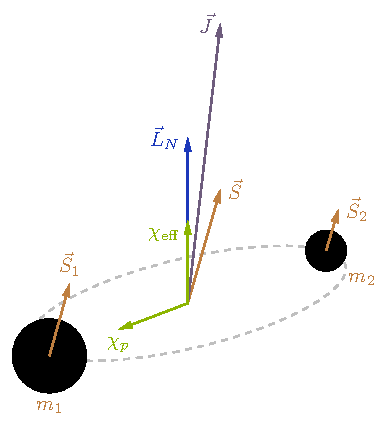
\includegraphics[width=0.4\textwidth]{examples/source_frame.pdf}}
    %
    \subfloat{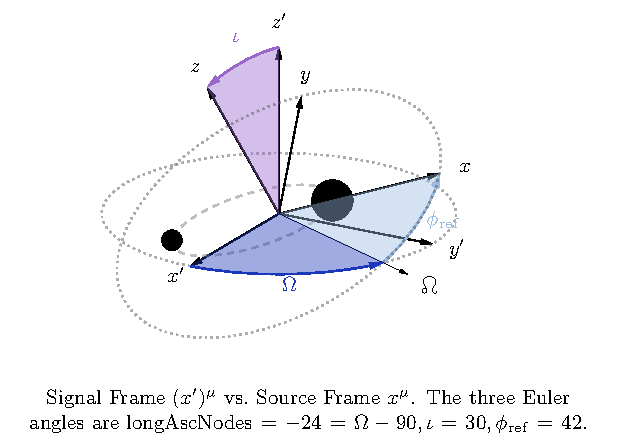
\includegraphics[width=0.6\textwidth]{examples/signal_frame.pdf}}

    \caption{Examples of frames that can be drawn with the \code{cbc\_frames\_tikz} package: source frame (top) and signal frame (bottom). For more details on how to create such plots, refer to the examples folder.}

    \label{fig:examples}
\end{figure}



    \section{List Of Keyword Arguments}
All three packages and their respective commands rely on \code{pgfkeys} to pass keyword arguments for customization. More specifically, there is a main \code{/frames} family with several sub-families. Here is a quick primer on how pgfkey families are used throughout the packages: When calling \code{\string\drawframes[argument=value]}, you pass \code{argument} to \code{/frames}; When calling \code{\string\drawframes[subfamily={argument=value,argument2=value2}]}, on the other hand, \code{argument} is passed to \code{/frames/subfamily}. For more details on the usage of sub-families etc.~in the actual commands, please refer to the examples folder (especially the \href{https://github.com/MaxMelching/gwframes/tree/main/examples/tutorials.tex}{tutorials file}).


In the following, we list all available keyword arguments for each family, along with their default values and short descriptions. For many of those keywords, there is more than one way in which they can be passed (for the \code{distance} argument, for example, there are the keys \code{/frames/distance} and \code{/frames/binary/distance}, and \code{/frames/distance/value}).\\


\emph{Note} that certain values cannot be passed to \code{pgfkeys}, which is particularly relevant for declaration of labels. If you encounter an issue of this kind, look up the command that this key is stored in (typically something like \code{\string\cbcframes@<parameter>@Label}), and manually set the command. This can be done using \code{\string\def\string\cbcframes@<parameter>@Label\{<input>\}}.\footnote{Depending on where you call that, do not forget to surround this with \code{\string\makeatletter \dots \string\makeatother}!} A practical example would be \code{\string\def\string\cbcframes@Omega@Label\{\$\string\Omega = \string\pi/2 + \string\mathrm\{longAscNodes\}\$\}}.


\emph{Also note} that all angles are expected to be given in degrees.



        \subsection{\texttt{cbc\_frames\_tikz}}\label{sec:cbc_frames_tikz}
The sub-families introduced here usually accept a family of keyword arguments, i.e.~input like \code{\string\drawframes[sourceframe={mass1=20,mass2=10}]}. However, for most of them it is also possible to pass a single argument, which is passed on to a sensible keyword of that family (if, for instance, \code{\string\drawframes[inclination=42]} is called, then $42$ is passed to \code{/frames/inclination/value}; for \code{\string\drawframes[celestialframe=false]}, it would be \code{/frames/celestialframe/show}, etc.); this keyword is stated at the end of the description of each sub-family.


\begin{itemize}
    \setlength{\itemsep}{10pt}

    \item \code{/frames/binary} family: Properties of the binary system.

    \begin{itemize}
        \item \code{show}: Whether to show the binary system.

        \defaultval{true}


        \item \code{mass1}: Mass of the first compact object, determining its size through multiplication by \code{bhsizepersolmass}.

        \defaultval{$20$}

        \separatepassing{/frames}


        \item \code{mass2}: Mass of the second compact object, determining its size through multiplication by \code{bhsizepersolmass}.

        \defaultval{$20$}

        \separatepassing{/frames}


        \item \code{eccentricity}: Determines the circularity of the binary black hole orbit

        \defaultval{$0$}

        \separatepassing{/frames}


        \item \code{separation}: Distance of binary companions, in multiples of \code{axislen}.

        \defaultval{$0.5$}


        \item \code{distance}: Distance of binary center of mass from Earth, in multiples of the axis length \code{axislen}.

        \defaultval{$3$}

        \separatepassing{/frames}

        \separatepassing{/frames/distance}


        \item \code{bhsizepersolmass}: Size of each black hole per solar mass.

        \defaultval{$\frac{0.35}{10}$}

        \separatepassing{/frames}
    \end{itemize}

    \defaultkw{show}


    \item \code{/frames/sourceframe}: (Mostly styling) Properties of the source frame.

    \begin{itemize}
        \item \code{show}: Whether to show the source frame. Has precedence over other commands for the styling of the source frame, such as \code{sourceframe/axes}.

        \defaultval{true}


        \item \code{axes}: Whether to show the source frame axes.

        \defaultval{true}


        \item \code{helperlines}: Whether to show the source frame helper lines.

        \defaultval{true}
    \end{itemize}

    \defaultkw{show}


    \item \code{/frames/signalframe}: (Mostly styling) Properties of the signal frame.

    \begin{itemize}
        \item \code{show}: Whether to show the signal frame. Has precedence over other commands for the styling of the signal frame, such as \code{signalframe/axes}.

        \defaultval{true}


        \item \code{axes}: Whether to show the signal frame axes.

        \defaultval{true}


        \item \code{helperlines}: Whether to show the signal frame helper lines.

        \defaultval{true}


        \item \code{angles}: Whether to visualize the signal frame angles.

        \defaultval{true}


        \item \code{showazimuthalangle}: Determines if a specific azimuthal angle used in \href{https://www.nature.com/articles/s41550-025-02632-5}{this} paper is visualized.

        \defaultval{false}

        \separatepassing{/frames}

        \separatepassing{/frames/azimuthalangle}
    \end{itemize}

    \defaultkw{show}


    \item \code{/frames/celestialframe}: (Mostly styling) Properties of the celestial frame.

    \begin{itemize}
        \item \code{show}: Whether to show the celestial frame. Has precedence over other commands for the styling of the celestial frame, such as \code{celestialframe/axes}.

        \defaultval{true}


        \item \code{axes}: Whether to show the celestial frame axes.

        \defaultval{true}


        \item \code{helperlines}: Whether to show the celestial frame helper lines.

        \defaultval{true}


        \item \code{angles}: Whether to visualize the celestial frame angles.

        \defaultval{true}
    \end{itemize}

    \defaultkw{show}


    \item \code{/frames/earth}: Properties of the Earth drawing.

    Accepts any keyword argument that can be passed to the \code{earth\_tikz} package (cf.~Sec.~\ref{sec:earth_tikz}). There is a slight change in the defaults, though, radius has a default value of $1.25$ here.

    \defaultkw{radius}

    \textit{Note} that the Earth is only shown if the celestial frame is shown.


    \item \code{/frames/ifo}: Properties of the interferometer on Earth.

    \begin{itemize}
        \item \code{show}: Whether to draw the interferometer.

        \defaultval{true}


        \item \code{armlength}: Arm length of the interferometer.

        % \defaultval{$\SI{2}{\centi\metre}$}
        \defaultval{$2$}
    \end{itemize}

    \defaultkw{show}

    \textit{Note} that the interferometer is only shown if the celestial frame is shown.


    \item \code{/frames/labels}: A centralized way to pass labels for various angles and other quantities. For virtually all of them, there is at least one other way to change the label, namely redefining the corresponding command (which is described in more detail above, at the beginning of this section); for several, there is also a separate keyword sub-family, a list of which is provided further below. Labels in this family are:

    \begin{itemize}
        \item \code{inclination}

        \item \code{polarization}

        \item \code{longascnodes}

        \item \code{omega}

        \item \code{phiref}

        \item \code{ra}

        \item \code{dec}

        \item \code{lineofsight}

        \item \code{distance}

        \item \code{ascnode}

        \item \code{azimuthalangle}
    \end{itemize}

    \defaultkw{}


    \item \code{/frames/angles}: A centralized way to pass values for various angles. For several of them, there is another way to change the value, namely passing it to a separate keyword sub-family, a list of which is provided further below. Angles in this family are:

    \begin{itemize}
        \item \code{inclination}

        \item \code{polarization}

        \item \code{longascnodes}

        \item \code{phiref}

        \item \code{ra}

        \item \code{dec}
    \end{itemize}

    \defaultkw{}


    \item \code{axislen}: Length of the axes of each coordinate system.

    % \defaultval{$\SI{3}{\centi\metre}$}
    \defaultval{$3$}


    \item \code{axislabelpad}: How far from the axis label is drawn from the axis arrow tip, in multiples of \code{axislen}.

    \defaultval{$0.12$}


    \item \code{/frames/inclination}

    \begin{itemize}
        \item \code{value}: Inclination between orbital plane ($x$-$y$-plane of the source frame) and sky plane ($x$-$y$-plane of the signal frame). This rotation is about the ascending node $\ascnode$.

        \defaultval{$0$}

        \item \code{show}: Whether to show the inclination angle.

        \defaultval{true}


        \item \code{label}: Label for the inclination angle.

        \defaultval{$\iota$}
    \end{itemize}

    \defaultkw{value}


    \item \code{/frames/polarization}

    \begin{itemize}
        \item \code{value}: Polarization angle, i.e. rotation of the $x$-axis in the sky plane (about the line of sight, which coincides with the $z$-axis of the signal frame).

        \defaultval{$0$}


        \item \code{show}: Whether to show the polarization angle.

        \defaultval{true}


        \item \code{label}: Label for the polarization angle.

        \defaultval{$\psi$}
    \end{itemize}

    \defaultkw{value}


    \item \code{/frames/longascnodes}

    \begin{itemize}
        \item \code{value}: Determines the angle between $x$-axis of the signal frame and the ascending node $\ascnode$. This angle is $\Omega = 90 + \mathrm{longAscNodes}$.

        \defaultval{$0$}


        \item \code{show}: Whether to visualize the longitude of the ascending node angle.

        \defaultval{true}


        % \item \code{label}: Label for the longitude of the ascending node angle.

        % \defaultval{$\mathrm{longAscNodes}$}


        \item \code{omegalabel}: Label for the angle that is derived from the longitude of the ascending node, i.e.~$\Omega = 90 + \mathrm{longAscNodes}$. This is the angle that is actually visualized.

        \defaultval{$\Omega$}
    \end{itemize}

    \defaultkw{value}


    \item \code{/frames/phiref}

    \begin{itemize}
        \item \code{value}: Reference angle $\phi_\mathrm{ref}$ that determines the rotation between ascending node and $x$-axis of the signal frame (about the inclined $z$-axis of the signal frame).

        \defaultval{$0$}


        \item \code{show}: Whether to visualize the reference angle.

        \defaultval{true}


        \item \code{label}: Label for the reference angle.

        \defaultval{$\phi_\mathrm{ref}$}
    \end{itemize}

    \defaultkw{value}


    \item \code{/frames/ra}

    \begin{itemize}
        \item \code{value}: Angle between Earth's $x$-axis and the projection of the line of sight onto Earth's equatorial plane.

        \defaultval{$0$}


        \item \code{show}: Whether to visualize the right ascension.

        \defaultval{true}


        \item \code{label}: Label for the right ascension.

        \defaultval{$\alpha$}
    \end{itemize}

    \defaultkw{value}


    \item \code{/frames/dec}

    \begin{itemize}
        \item \code{value}: Angle between line of sight and Earth's equatorial plane.

        \defaultval{$0$}


        \item \code{show}: Whether to visualize the declination.

        \defaultval{true}


        \item \code{label}: Label for the declination.

        \defaultval{$\delta$}
    \end{itemize}

    \defaultkw{value}


    \item \code{/frames/distance}

    \begin{itemize}
        \item \code{value}: Distance of the binary from Earth, in multiples of the axis length \code{axislen}.

        \defaultval{$3$}


        \item \code{show}: Whether to visualize the distance.

        \defaultval{true}


        \item \code{label}: Label for the distance.

        \defaultval{$D_L$}
    \end{itemize}

    \defaultkw{value}


    \item \code{/frames/lineofsight}

    \begin{itemize}
        \item \code{show}: Whether to visualize the line of sight.

        \defaultval{true}


        \item \code{label}: Label for the line of sight.

        \defaultval{$\vec{N}$}
    \end{itemize}

    \defaultkw{show}


    \item \code{/frames/ascnode}

    \begin{itemize}
        \item \code{how}: Whether to visualize the ascending node.

        \defaultval{true}


        \item \code{label}: Label for the ascending node.

        \defaultval{$\ascnode$}
    \end{itemize}

    \defaultkw{show}


    \item \code{/frames/azimuthalangle}

    \begin{itemize}
        \item \code{show}: Determines if a specific azimuthal angle used in \href{https://www.nature.com/articles/s41550-025-02632-5}{this} paper is visualized.

        \defaultval{false}


        \item \code{label}: Label for the azimuthal angle.

        \defaultval{\$\string\pi/2 - \$\string\cbcframes@PhiRef@Label}
        % \defaultval{{\ttfamily\$\string\Omega = \string\pi/2 + \string\mathrm\{longAscNodes\}\$\}}}  % Works only because of ttfamily (?!)
    \end{itemize}

    \defaultkw{show}


    % \item \code{uselayers}

\end{itemize}



        \subsection{\texttt{cbc\_binary\_tikz}}\label{sec:cbc_binary_tikz}
\code{pgfkeys} family: \code{/frames/binary}


\begin{itemize}
    % \setlength{\itemsep}{10pt}

    \item \code{mass1}: Mass of the first binary component, in solar masses.

    \defaultval{$20$}


    \item \code{mass2}: Mass of the second binary component, in solar masses.

    \defaultval{$10$}


    \item \code{spin1x}: $x$-component of the dimensionless spin of the first binary component.

    \defaultval{$0$}


    \item \code{spin1y}: $y$-component of the dimensionless spin of the first binary component.

    \defaultval{$0$}


    \item \code{spin1z}: $z$-component of the dimensionless spin of the first binary component.

    \defaultval{$0$}


    \item \code{spin2x}: $x$-component of the dimensionless spin of the second binary component.

    \defaultval{$0$}


    \item \code{spin2y}: $y$-component of the dimensionless spin of the second binary component.

    \defaultval{$0$}


    \item \code{spin2z}: $z$-component of the dimensionless spin of the second binary component.

    \defaultval{$0$}


	\item \code{inclination}: Inclination of the orbital plane with respect to the $xy$-plane. (The orbital plane is the plane in which the two binary components orbit each other.)

    \defaultval{$0$}


	\item \code{polarization}: Angle or rotation in the orbital plane.

    \defaultval{$0$}


    \item \code{eccentricity}: How eccentric the binary orbit is.

    \defaultval{$0$}


    \item \code{separation}: How far the binary components are separated.

    \defaultval{$6$}


    \item \code{showcombinedquantities}: Whether to show quantities like the effective or precessing spin, which are combinations of the properties of both binary components.

    \defaultval{true}
\end{itemize}

Other quantities of interest are the two commands \code{\string\cbcframes@BHsizepersolmass} and \code{\string\cbcframes@UnitSpinSize}, which determine the sizes of black holes and spins, respectively.



        \subsection{\texttt{earth\_tikz}}\label{sec:earth_tikz}
\code{pgfkeys} family: \code{/frames/earth}


\begin{itemize}
    % \setlength{\itemsep}{10pt}

    \item \code{radius}: Radius of the Earth

    \defaultval{$1$}


    \item \code{tilt}: Tilt of the Earth

    \defaultval{$0$}
\end{itemize}



\end{document}
